\section{Kết luận và hướng nghiên cứu tiếp theo (Conclusion and Future Work)}
\label{sec:conclusion}

\subsection{Kết luận Toàn diện (Conclusion)}
Bài báo này đã giải quyết trọn vẹn bài toán Dự báo Phụ tải Điện Ngắn hạn theo giờ (STLF) trên lưới điện thực tế của Công ty Điện lực và Khí đốt Thái Bình Dương (PG\&E), thuộc khuôn khổ cuộc thi học thuật \textit{IISE PG\&E Energy Analytics Challenge 2025}.

Khởi đầu từ việc tái lập nghiêm ngặt công trình đối chuẩn của Roy, Pyltsov và Hu~\cite{roy2025hourly}, chúng tôi đã xác thực luận điểm thực nghiệm quan trọng: các mô hình học máy dạng bảng phân đoạn theo giờ (24-Hourly XGBoost) sở hữu ưu thế vượt trội so với các kiến trúc Deep Learning Transformers phức tạp trong bài toán STLF thực tế. Tuy nhiên, bằng việc phân tích sâu sắc các hạn chế cố hữu về mặt vật lý công trình và cấu trúc mô hình đơn lẻ của bài báo gốc, nhóm nghiên cứu đã mở rộng và thiết lập một khung phương pháp ensemble mới với ba đóng góp đột phá:
\begin{enumerate}
    \item \textbf{Kỹ nghệ Đặc trưng Định hướng Vật lý (Physics-Informed Features):} Bổ sung các chỉ số ngưỡng nhiệt động lực học $\text{HDD}$ và $\text{CDD}$ dựa trên nhiệt độ cơ sở tiện nghi $18^\circ\text{C}$ chuẩn ASHRAE, kết hợp cùng chuỗi điều hòa Fourier liên tục theo chu kỳ nhật triều và chu kỳ năm thiên văn. Việc tích hợp này giúp làm mượt các bước nhảy giả tạo của biến tháng và đưa vào tín hiệu kích hoạt phi tuyến sắc nét của hệ thống làm mát HVAC, giúp giảm ngay $11.01$~MW sai số RMSE so với baseline tái lập ($10.19$~MW so với baseline bài báo gốc).
    \item \textbf{Khám phá Hiện tượng Chế độ Vận hành Kép (Dual-Regime Discovery):} Lần đầu tiên phát hiện và chứng minh định lượng tính bù trừ sai số mạnh mẽ giữa mô hình tuyến tính ElasticNet (L1/L2 regularization) và mô hình phi tuyến dạng cây XGBoost với hệ số tương quan phần dư chỉ đạt $r = 0.6131$. Chúng tôi chứng minh sự phân tầng rõ rệt: ElasticNet vượt trội hơn trong chế độ phụ tải nền ban đêm (\textit{nocturnal baseload}, 00:00--06:00: RMSE $131.33$~MW so với $141.37$~MW), trong khi XGBoost chiếm ưu thế áp đảo trong chế độ sóng nhiệt mùa hè (\textit{summer heatwaves}, CDD $> 3^\circ\text{C}$: RMSE $244.16$~MW so với $313.27$~MW).
    \item \textbf{Kiến trúc Context-Aware Stacking (CAS):} Phát triển mô hình meta-learner LightGBM được điều hòa đồng thời bởi dự báo của các mô hình cơ sở (\textit{base models}) và vector ngữ cảnh khí tượng -- thời gian thực. Hoạt động như một bộ định tuyến thích nghi động (\textit{dynamic router}), CAS đạt kỷ lục mới với RMSE \textbf{141.81~MW}, MAPE \textbf{4.75\%}, và $R^2$ \textbf{0.9136} trên tập kiểm tra độc lập Year 3 (2022). So với baseline của bài báo gốc ($170.84$~MW), mô hình CAS đề xuất giúp cắt giảm tới \textbf{$-$29.03~MW} (tương đương \textbf{$-$17.0\% RMSE}).
\end{enumerate}

Toàn bộ quy trình ra quyết định đã được kiểm chứng và giải thích minh bạch qua biểu đồ nhiệt SHAP 24 giờ, cung cấp cơ sở tin cậy tuyệt đối cho các kỹ sư điều độ hệ thống điện.

\subsection{Hướng Nghiên cứu Tiếp theo (Future Work)}
Từ các kết quả và hạn chế đã chỉ ra, nhóm định hướng bốn hướng nghiên cứu mở rộng đầy tiềm năng trong tương lai:
\begin{enumerate}
    \item \textbf{Định lượng Độ Bất định với Conformal Prediction Thích nghi Thời gian (\textit{Time-Adaptive Conformal Prediction}):}
    Bên cạnh dự báo điểm (\textit{point forecast}), các nhà điều hành hệ thống điện rất cần các khoảng tin cậy khả tín (\textit{prediction intervals}) với bảo đảm bao phủ thống kê không phụ thuộc phân phối (\textit{distribution-free coverage guarantee}) theo lý thuyết của Vovk et al.~\cite{vovk2005algorithmic}. Nhóm đã bước đầu thử nghiệm trích xuất các khoảng tin cậy $95\%$ bằng Conformal Prediction (Hình~\ref{fig:cp_intervals}) và sẽ tiếp tục phát triển thuật toán tự động hiệu chỉnh độ rộng khoảng tin cậy theo phương sai thời tiết thời gian thực.

    \begin{figure}[htbp]
        \centering
        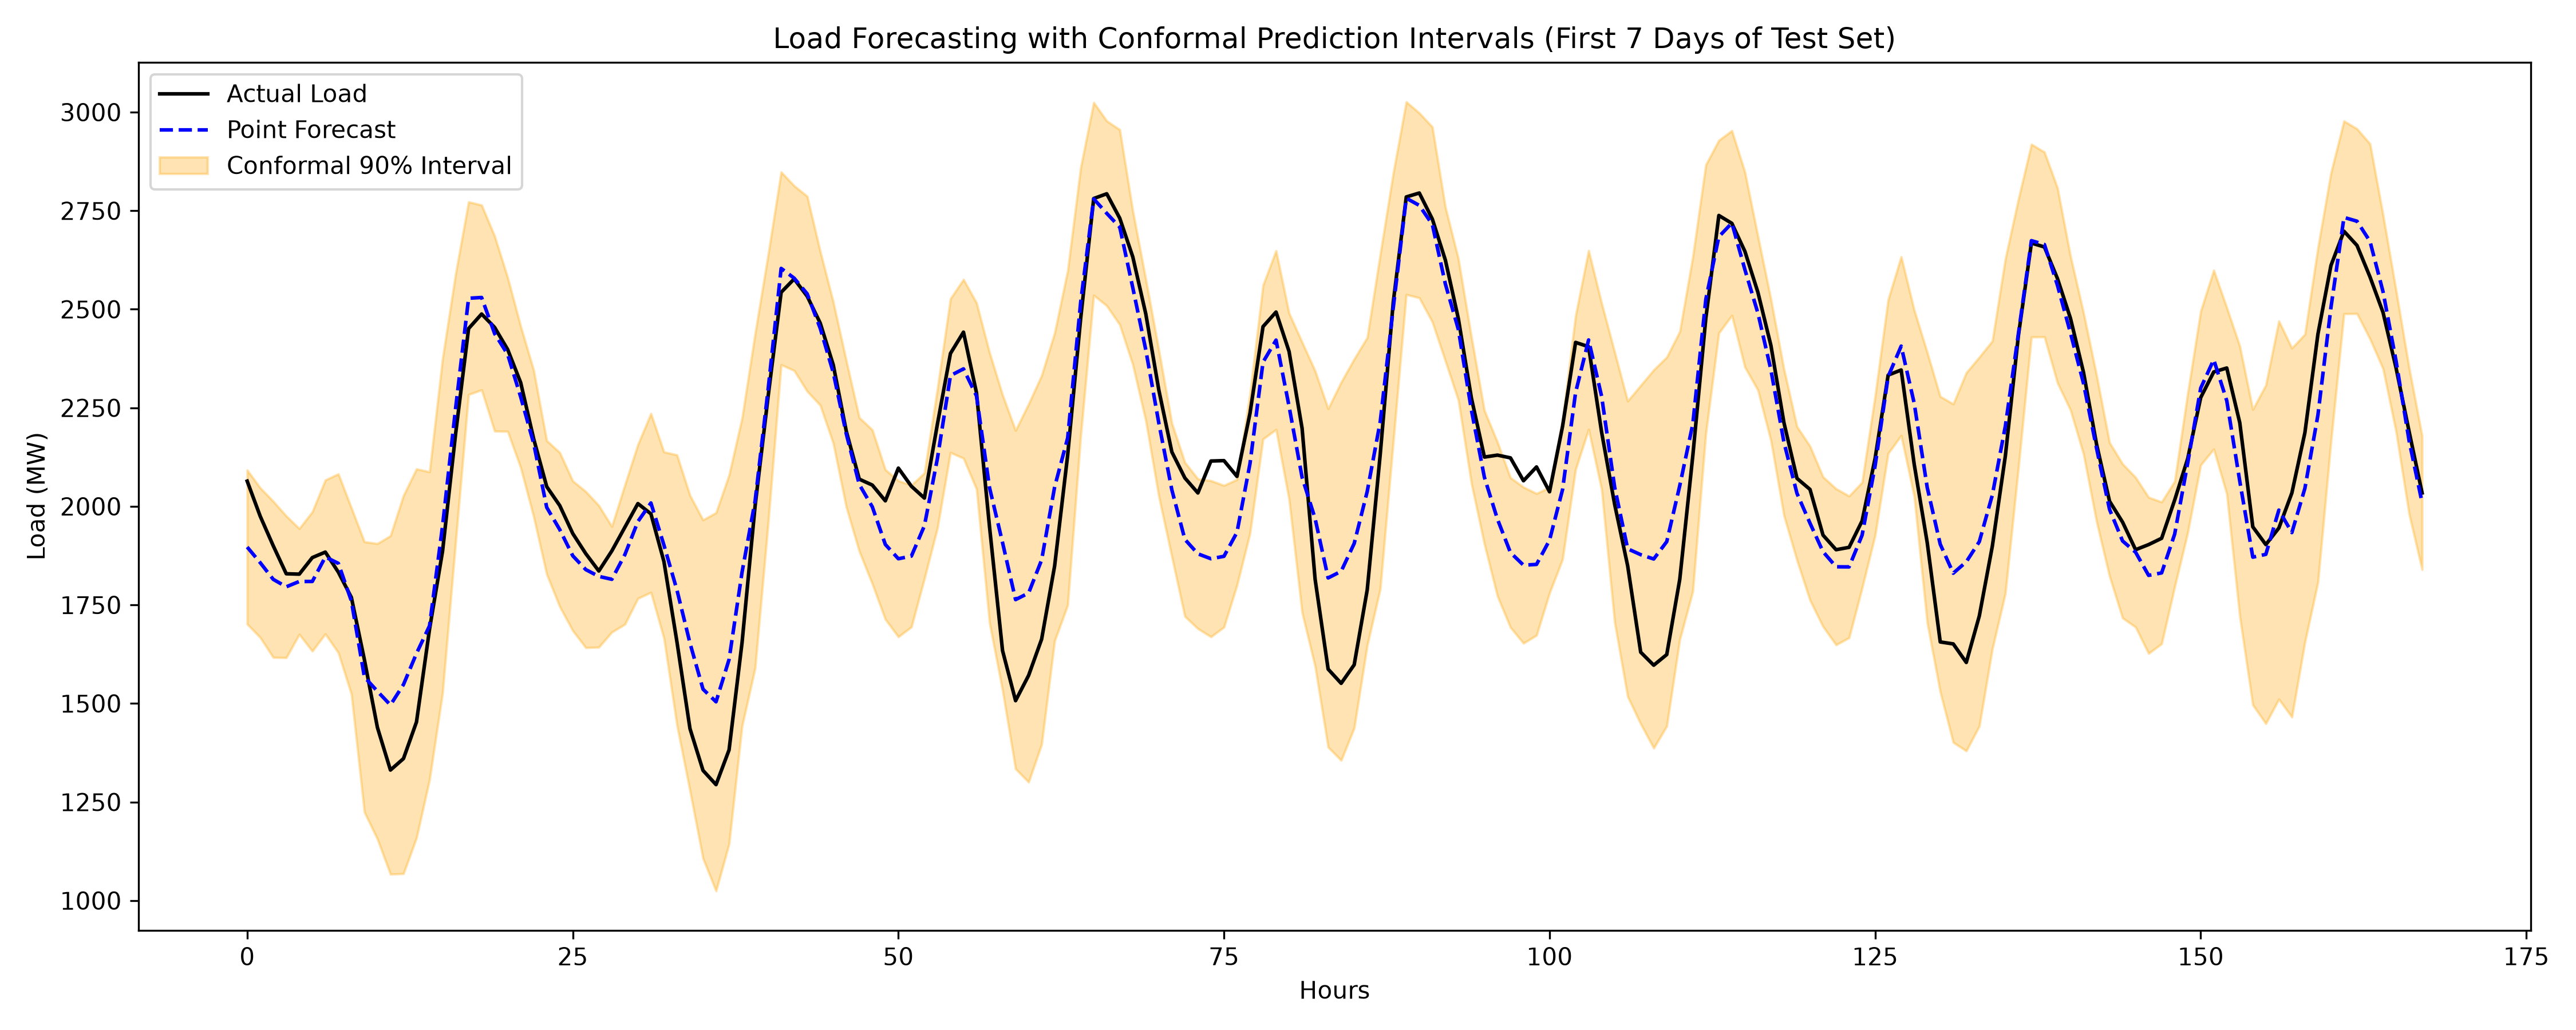
\includegraphics[width=0.95\textwidth]{figures/fig_cp_intervals.png}
        \caption{Khoảng Dự báo Tin cậy 95\% bằng Conformal Prediction trên Chuỗi Phụ tải PG\&E.}
        \label{fig:cp_intervals}
    \end{figure}

    \item \textbf{Mở rộng Kiểm chứng Đa Lưới điện (\textit{Multi-Grid Benchmark}):}
    Đánh giá tính khái quát hóa của khung phương pháp CAS trên các thị trường điện quy mô lớn khác tại Bắc Mỹ như PJM Interconnection, ERCOT (Texas), NYISO (New York) và toàn bộ vùng CAISO (California) nhằm thẩm định khả năng thích nghi với các vùng khí hậu và cơ cấu phụ tải khác nhau.
    \item \textbf{Mô hình hóa Quán tính Nhiệt Đa ngày và Chỉ số Khí quyển Bổ sung:}
    Tích hợp các biến trễ nhiệt độ tích lũy từ 3 đến 5 ngày trước đó nhằm khắc phục triệt để hiện tượng "ngậm nhiệt" của bê tông đô thị trong các đợt sóng nhiệt kéo dài; đồng thời thu thập thêm các biến độ ẩm không khí và tốc độ gió để tính toán chỉ số nhiệt cảm nhận (\textit{Heat Index}).
    \item \textbf{Tích hợp Phụ tải Điện Mặt trời Mái nhà và Trạm Sạc Xe điện (EV):}
    Phát triển các mô hình nhánh chuyên biệt để phân rã ảnh hưởng của điện mặt trời mái nhà tự dùng và nhu cầu sạc xe điện ban đêm, nhằm đáp ứng mục tiêu phát thải ròng bằng 0 (\textit{Net Zero}) của các lưới điện tương lai.
\end{enumerate}
